\chapter{Static Analysis (partly READY FOR FEEDBACK, PROOFREAD)}
\label{static-analysis}

This chapter describes static code analysis, the difference to other analysis types, the technical details and the theory behind it.

\section{Static Analysis vs.~Dynamic Analysis}

Generally, there are two basic approaches to program analysis, differentiated by the time the analysis is performed: \emph{static analysis} and \emph{dynamic analysis}.

\subsection{Static Analysis}
\index{static analysis}\index{SA\see{static analysis}}\index{static code analysis|see{static analysis}}

\emph{Static analysis (SA)} or \emph{Static code analysis} is defined as analyzing the way code of a program (the source code, byte code or machine code) will execute instead of---or before---actually running it. The analysis is performed on an abstract level, \ie it does not use concrete data for checking.~\cite{static-code-analysis}

The aim of static analysis is to find bugs, structural problems, code smells or to help in understanding the system that is analyzed very early in the development cycle.~\cite{data-flow-analysis, chess-west} Optimally, the developer will be able to see the problems directly during development, \eg as markers in their development environment, or as feedback from a tool that is run in parallel.

Static analysis allows all possible program paths to be checked, independent of the program paths actually being executed during the particular set of data used during execution. In addition, the results of static code analysis are repeatable.~\cite{coverity-report}

\subsection{Dynamic Analysis}
\index{dynamic analysis}

\emph{Dynamic analysis} is code analysis that happens when the code is executed. This usually comes with a performance penalty, but it also increases precision because the analysis works on the actual data instead of a general model of the data.~\cite{chess-west} However, it also considerably reduces the callback as the dynamic analysis always works on a concrete set of data, and the analysis will not find problems that only occur with different data.~\cite{static-code-analysis}

Examples of automated dynamic analysis would be penetration tests for the outside view or unit tests.



\section{Approaches to Static Analysis}
Generally, there are several different approaches when doing static code analysis~\cite{comparison-of-bug-finding-tools}: string pattern matching, syntactic bug pattern detection, data-flow analysis, theorem proving and model checking, all of which are to be explained in this section.


\subsection{String Pattern Matching}
\index{string pattern matching}

\emph{String pattern matching} is the most simple form of static code analysis.

With this ap\-proach, the scanner approaches the source code basically just as list of lines, which consist of characters. This kind of scanner does not operate on tokens or any other abstracted structure of the program.

To the author's knowledge, this approach is only used in security scanners, but not for other static code analysis tools.

The scanner checks for security vulnerabilities by scanning for certain commands or command sequences and heavily relies on the human eye for filtering out false positives. This greatly reduces its practical use as programmers tend to ignore warnings if they contain lots of false positives.~\cite{understanding-value}

Still, it is possible to use this approach for finding some vulnerabilities, for example using \emph{Google Code Search}\index{Google Code Search}.~\cite{google-code-search}

The main drawback of this approach is that there are lots of false positives (\eg with the tool SWAAT~\cite{swaat}) as the tools do not use any data-flow analysis and thus cannot distinguish between a potentially unsafe command being executed with data that is in fact unsafe and those cases where the data is already ensured to be safe at that point.

The most basic way of applying this code analysis is by simply using the text search function of a text editor---possibly with regular expressions\index{regular expressions}---or text-search command line tools like \emph{grep}.


\subsection{Syntactic Bug Pattern Detection (``Style Checking'')}
\index{style checking}\index{syntactic bug pattern detection}

Syntactic bug pattern detection means the scanner works a model of the code and its structure, for example a stream of tokens or an abstract syntax tree (section~\ref{ast}). However, this kind of scanner does not apply any interprocedural control-flow or data-flow analysis. This type of scanner often is used for enforcing coding style guidelines, \eg in continuous integration (CI)\index{continuous integration} environments like \emph{Jenkins}~\cite{jenkins}. Hence, these scanners also are called ``style checkers''.

Compared to string pattern matching for finding bugs, this approach greatly reduces the number of false positives and makes the scanner a lot more useful.~\cite{comparison-of-bug-finding-tools}. Tools like \emph{PHPCodeSniffer}\index{PHPCodeSniffer}, \emph{PMD}\index{PMD} or \emph{FindBugs}\index{FindBugs} fall into this category.


\subsection{Data-Flow Analysis}
\index{data-flow analysis}\index{control-flow analysis}

Scanners that rely on data-flow analysis first create information about the control flow, \ie about the possible paths through the program. On top of this information, they compute information about what data is used or modified at which program point.~\cite{data-flow-analysis} This information usually is an approximation of the real data that is used during program execution.

Data flow analysis consists of \emph{intraproceducal data-flow analysis}\index{intraproceducal data-flow analysis} (\ie the analysis of the data flow both within a function as well as in the global scope) and \emph{interproceducal data-flow analysis}\index{interproceducal data-flow analysis}, \ie the analysis of the data flow between functions.

Data-flow analysis is the most precise way of scanning statically for security vulnerabilities without having to annotate the source code in any way.~\cite{comparison-of-bug-finding-tools}

\emph{Pixy}~\cite{pixy} is an example of a security scanner using data-flow analysis.


\subsection{Theorem Proving}
\index{theorem proving}

\emph{Theorem proving} relies on the programmer adding preconditions, postconditions and loop invariants to the source code as code annotations. The scanner then can analyze the program and check whether all conditions are met.~\cite{comparison-of-bug-finding-tools}

\emph{ESC/Java}\index{ESC/Java} is an example from this class of tools.


\subsection{Model Checking}
\index{model checking}

Model checking relies on creating suitable models of the program---either manually or automatically by using code annotations that state what should be checked.~\cite{data-flow-analysis} One drawback of this class of scanners is that programs including library calls are practically impossible to check as it would be necessary to model their complete behavior, not just \eg the fact that they do (or do not) sanitize their inputs. This greatly reduces the 	feasibility of this approach for real-world programs.~\cite{comparison-of-bug-finding-tools}

\emph{Bandera}\index{Bandera} is a scanner that makes use of model checking.



\section{The Components of a Code Analyzer using Data-flow Analysis}

The components at the start of the processing chain of a code analyzer using data-flow analysis basically are the same components that compilers use (figure~\ref{fig:compiler-parts} on page~\pageref{fig:compiler-parts}). The reason for this is that both static code analyzers and compilers can start with the source code as a plain text file and need some abstract semantic information on the program to work with.

If the static code analyzer works on a later product of the compiler tool chain (such as bytecode or machine code), the static code analyzer of course does not need to have the components that already have been used by the compiler. For example, JLint works on Java bytecode~\cite{comparison-of-bug-finding-tools}, and Bytekit works on the bytecode generated during the PHP interpreter's compilation phase, providing control flow graphs.~\cite{bytekit, bytekit-cli}\index{bytecode}

\begin{figure}[htb]
  \begin{center}
    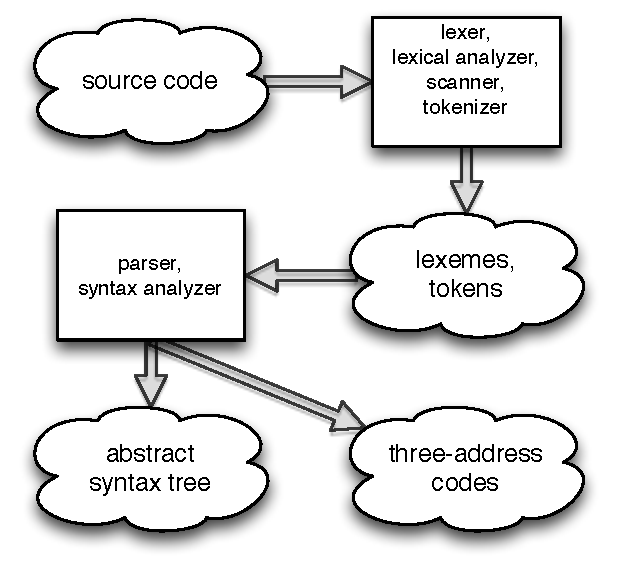
\includegraphics[scale=1.0]{images/compiler-parts}
    \caption{The main components in the processing chain of a code analyzer using data-flow analysis basically are the same as these from a compiler.}
    \label{fig:compiler-parts}
  \end{center}
\end{figure}


\subsection{Lexer, Lexical Analyzer, Scanner, Tokenizer}
\index{lexer}\index{lexical analyzer}\index{scanner}\index{tokenizer}\index{token manager}

The \emph{lexer} (also referred to as \emph{lexical analyzer}, \emph{scanner}\footnote{In all other places of this thesis, the author uses the term \emph{scanner} with the meaning ``security scanner''.} or \emph{tokenizer}) takes the stream of characters of the source program as input and converts them into meaningful sequences called \emph{tokens} or \emph{lexemes}.~\cite{compilers, compiler-construction}\index{token}\index{lexeme}


\subsection{Parser, Syntax Analyzer}
\index{parser}\index{syntax analyzer}

The \emph{parser}---also referred to as \emph{syntax analyzer}---takes the lexemes (tokens) as input and creates a tree-like intermediate representation for the grammatical structure of the to\-kens. This usually either is an abstract syntax tree (AST) or a three-address code (TAC).~\cite{compilers, compiler-construction}\index{abstract syntax tree}\index{AST\see{abstract syntax tree}}\index{three-address code}\index{TAC\see{three-address code}}


\section{Abstract Syntax Trees (AST) (READY FOR FEEDBACK)}
\label{ast}
\index{abstract syntax tree}\index{AST\see{abstract syntax tree}}

An \emph{abstract syntax tree (AST)}~\cite{compiler-construction} is an abstract representation of the structure of a program. This representation is stripped of anything that is not essential for the semantics of the program: For example, the tree does not contain parenthesis; instead, the order of execution is represented in the order and hierarchy of the tree. Thus, it is not possible to reconstruct the exact source code back from an abstract syntax tree, while it still is possible to rebuild a program that has the same semantics as the original program.

For the following code example, figure~\ref{fig:ast} on page~\pageref{fig:ast} shows the corresponding abstract syntax tree.

\begin{phpcode}
if ($x > $y) {
  $z = 42;
}
\end{phpcode}

An abstract syntax tree is still mostly human-readable \ldots if the reader knows how to read a tree using a pre-order walk.

\begin{figure}[htb]
  \begin{center}
    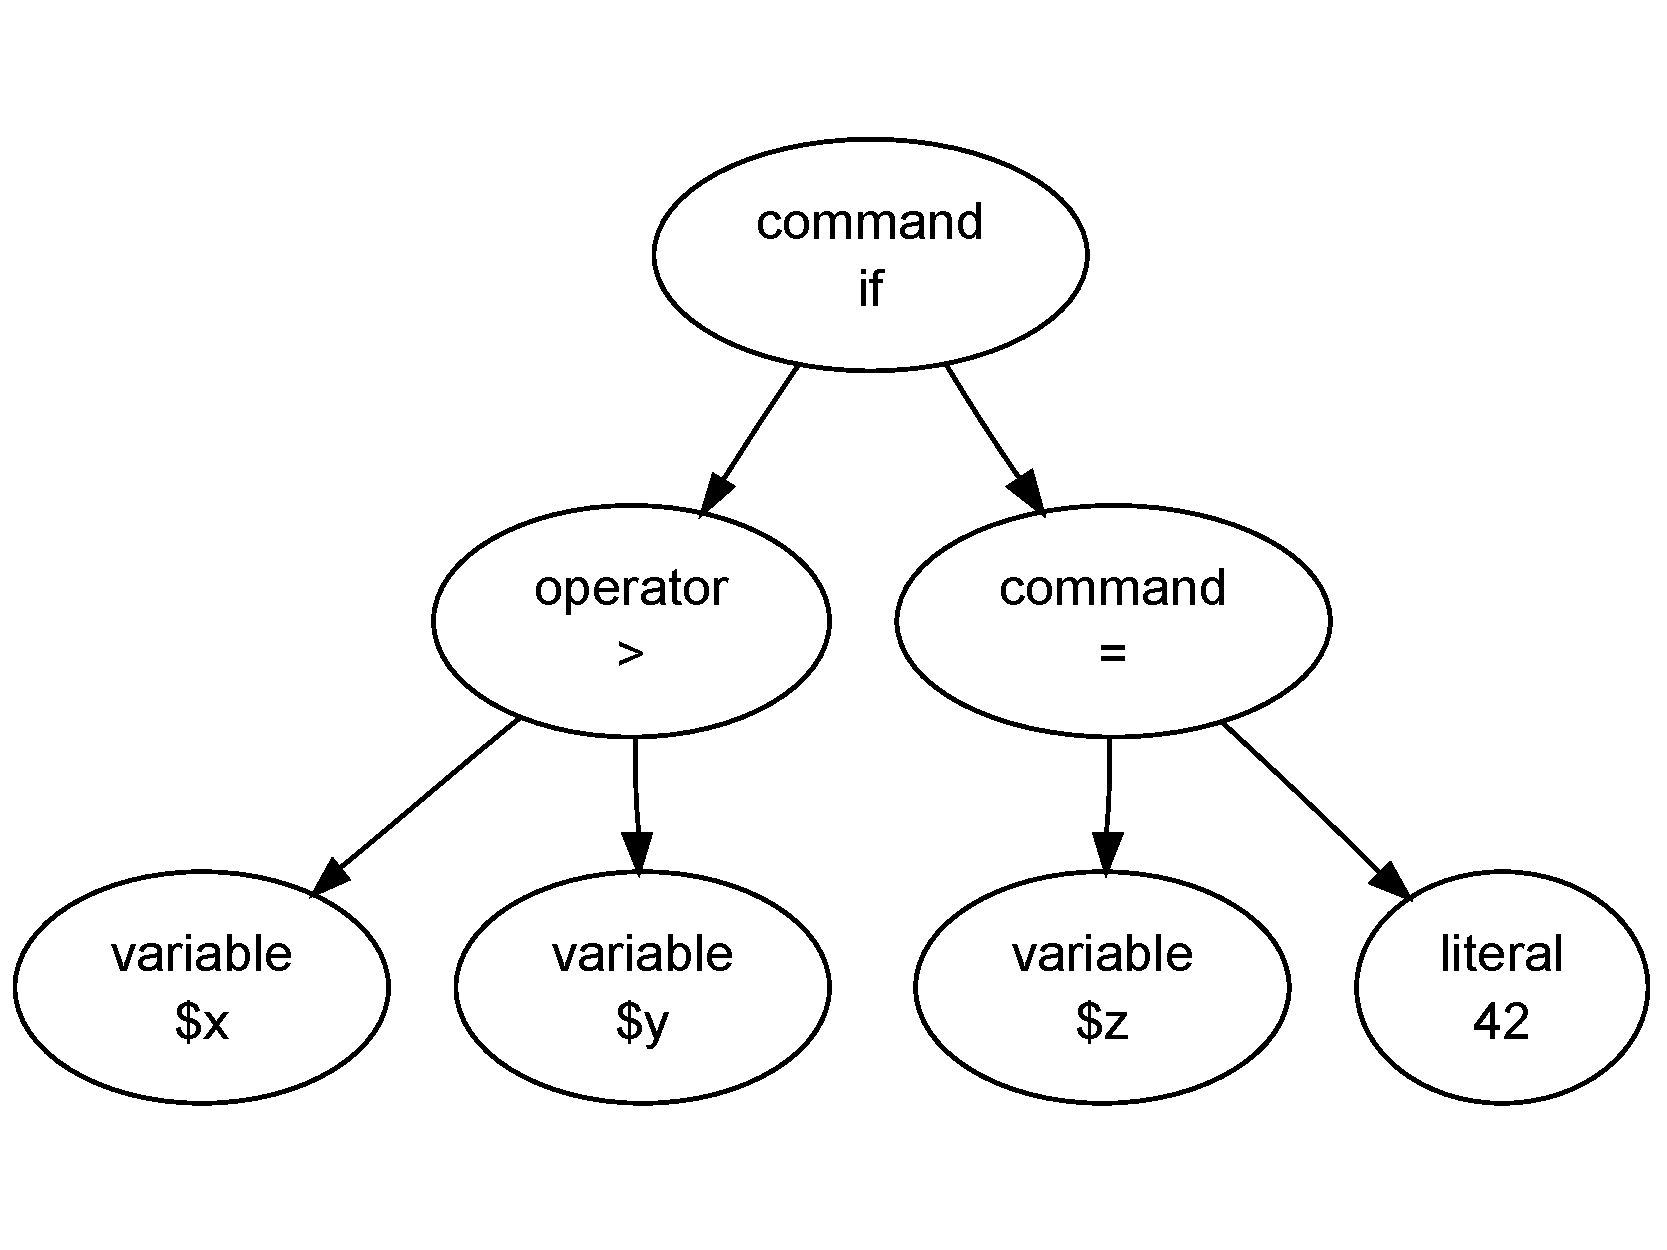
\includegraphics[scale=0.4]{images/ast}
    \caption{An abstract syntax tree (AST) represents the semantic structure of the original program, but does not contain the syntactic details.}
    \label{fig:ast}
  \end{center}
\end{figure}



\section{Parse Trees/Concrete Syntax Trees (READY FOR FEEDBACK)}
\label{parse-tree}
\index{parse tree}\index{concrete syntax tree}

A \emph{concrete syntax tree} or \emph{parse tree}~\cite{compiler-construction, compilers} contains all elements of the original source code in a semantic structure, including parenthesis, and comments. It is possible to fully reconstruct the original code from a parse tree---except for some indentation details---, making a parse tree also useful for transformations within the source code. On the downside, parse trees are very verbose in comparison to abstract syntax trees, which are reduced to the bare semantics.

For the following code example (which is the same as in section~\ref{ast}), figure~\ref{fig:parse-tree} on page~\pageref{fig:parse-tree} shows the corresponding PHP parse tree as created by the PhpParser package. The difference in size---for the exact same source code---is striking. The figure shows that the PHP opcodes also are listed with their opcode name, \eg \emph{T\_CLOSE\_BRACES}.

\begin{phpcode}
if ($x > $y) {
  $z = 42;
}
\end{phpcode}
\label{parsetree-code}

\begin{figure}[htb]
  \begin{center}
    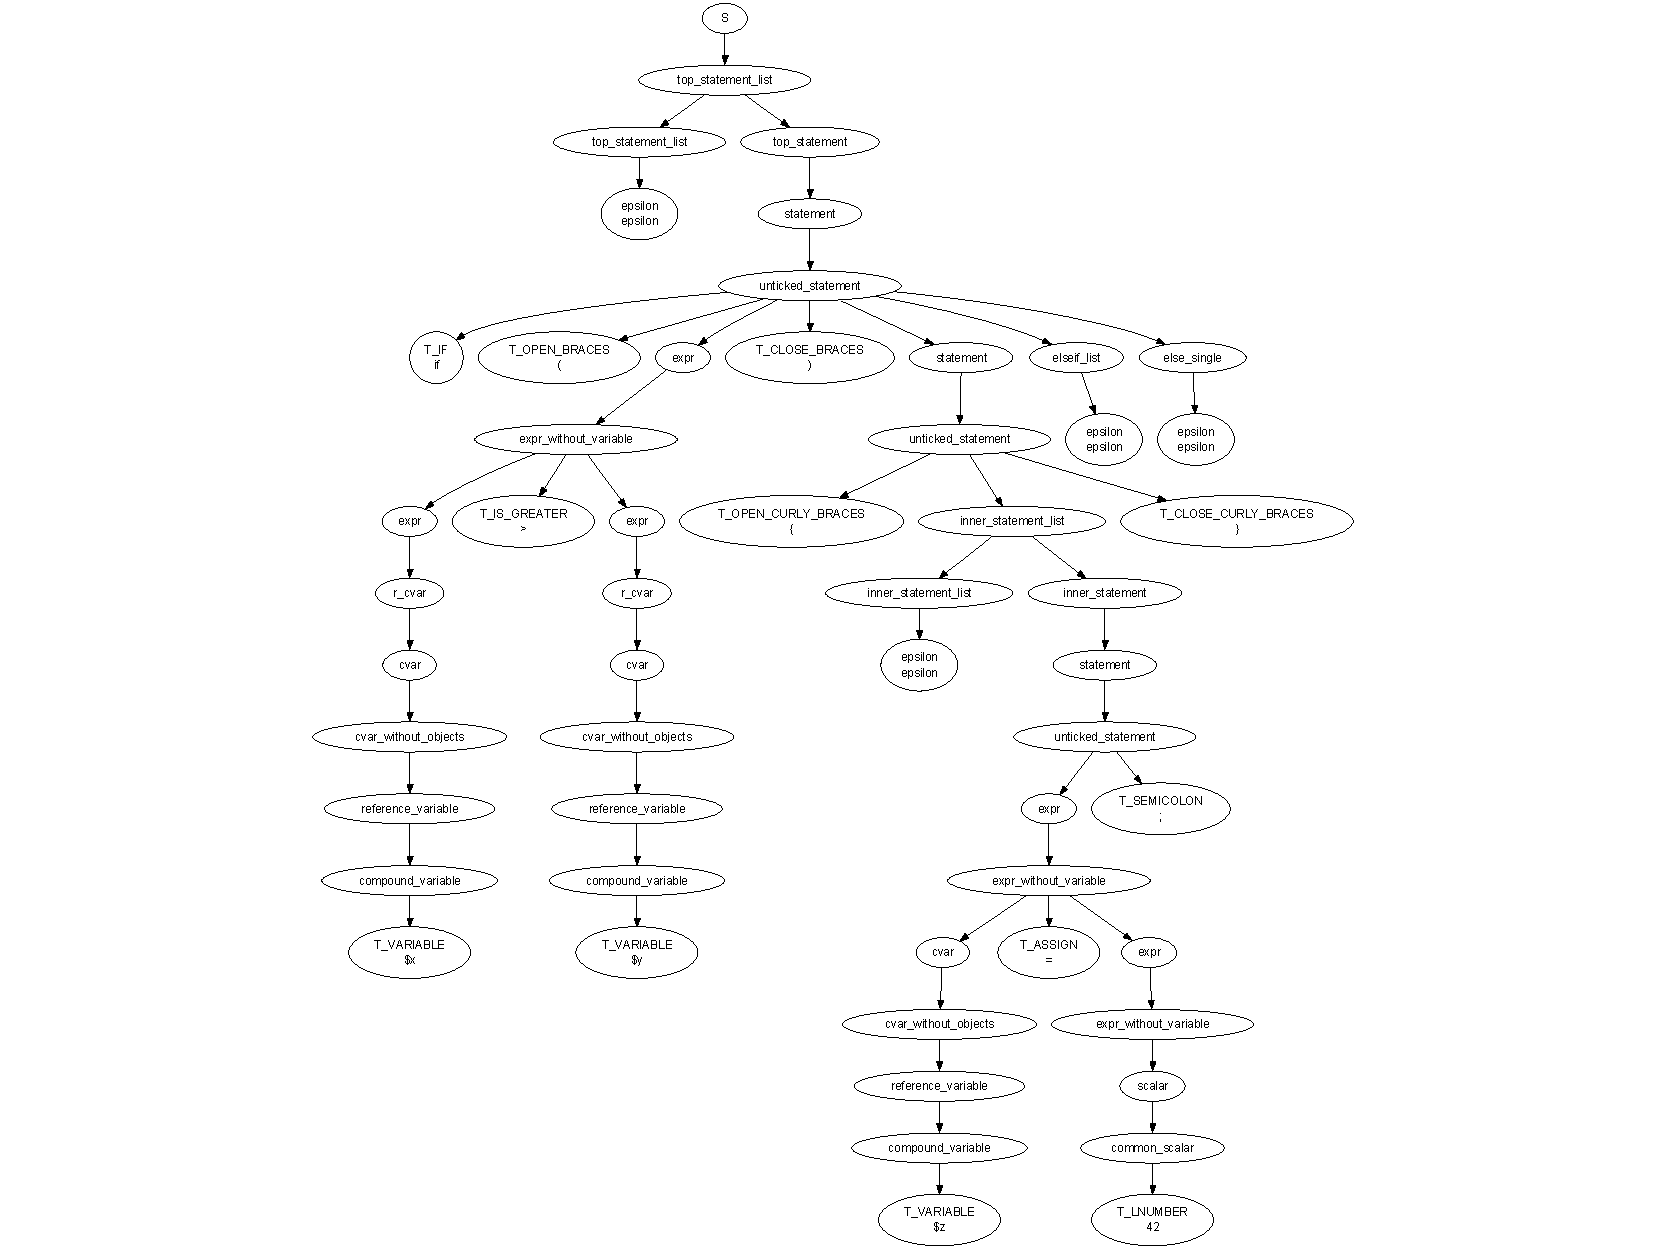
\includegraphics[scale=0.84, trim=54mm 0mm 0mm 0mm]{images/parse-tree}
    \caption{A parse tree contains all the syntactic details of the original code, making it extremely verbose. This is the PHP parse tree generated by PhpParser and Pixy from the small code example in section~\ref{parsetree-code} on page~\pageref{parsetree-code}.}
    \label{fig:parse-tree}
  \end{center}
\end{figure}



\section{Three-address Code (TAC) (READY FOR FEEDBACK)}
\label{tac}
\index{three-address code}\index{TAC\see{three-address code}}

\emph{Three-address code (TAC)}~\cite{compiler-construction, compilers} is a theoretical concept for an intermediate program representation that roughly resembles assembly code. Three-address codes each consist of a basic operation and up to three operands or eponymic ``addresses''. Addresses can be variables, constants, literals, compiler-generated temporaries, or jump targets.

Three-address code breaks down deep expressions and loops into a relatively simple, linearized structure with conditions and jumps, making it particularly useful for data-flow analysis.

Let's see how some example PHP code translates into three-address code:

\begin{phpcode}
$x = 1;
$y = 2;
$x = $x + $y + 3;
if ($x == 6) {
  $z = 4;
}
\end{phpcode}

There are two approaches to writing three-address code. The first approach lists the operator first, making the notation more strict:

\begin{textcode}
     (=, x, 1)            // x = 1
     (=, y, 2)            // y = 2
     (+, t0, x, y)        // t0 is a compiler-generated temporary as
                          // x gets overwritten, making x non-unique.
     (+, t1, t0, 3)       // t1 is another generated temporary.
     (if_neq, t1, 6, @L0) // Jumpo to @L0 if t1 is not equal to 6.
     (=, z, 4)            // z = 4
@L0:                      // The jump target is labelled @L0.
\end{textcode}

Another approach is to put the operator(s) where they fit more naturally, making the notation more human-readable:

\begin{textcode}
     (x = 1)
     (y = 2)
     (t0 = x + y)
     (t1 = t0 + 3)
     (if t1 != 6 goto @L0)
     (z = 4)
@L0:
\end{textcode}

This is still the same three-address code, just written a bit differently.



\section{Control-flow Graphs (READY FOR FEEDBACK)}
\label{cfg}
\index{control-flow graph}\index{CFG\see{control-flow graph}}\index{flow graphs\see{control-flow graphs}}

A \emph{control-flow graph (CFG)}~\cite{chess-west} or \emph{flow graph}~\cite{compilers} is a directed graph built on top of an abstract syntax tree or a parse tree that models the different paths through a program. Control-flow graphs are an important structure used in data-flow analysis.

Let's look at an example. For the following PHP code example, figure~\ref{fig:cfg} on page~\pageref{fig:cfg} depicts the corresponding control-flow graph. Note that the loop is changed to a conditional jump.

\begin{phpcode}
$count = 0;
$output = '';

while (strlen($output) < 99) {
  $output .= 'Hello world! ';
  $count++;
}

echo $output;
\end{phpcode}

\begin{figure}[htb]
  \begin{center}
    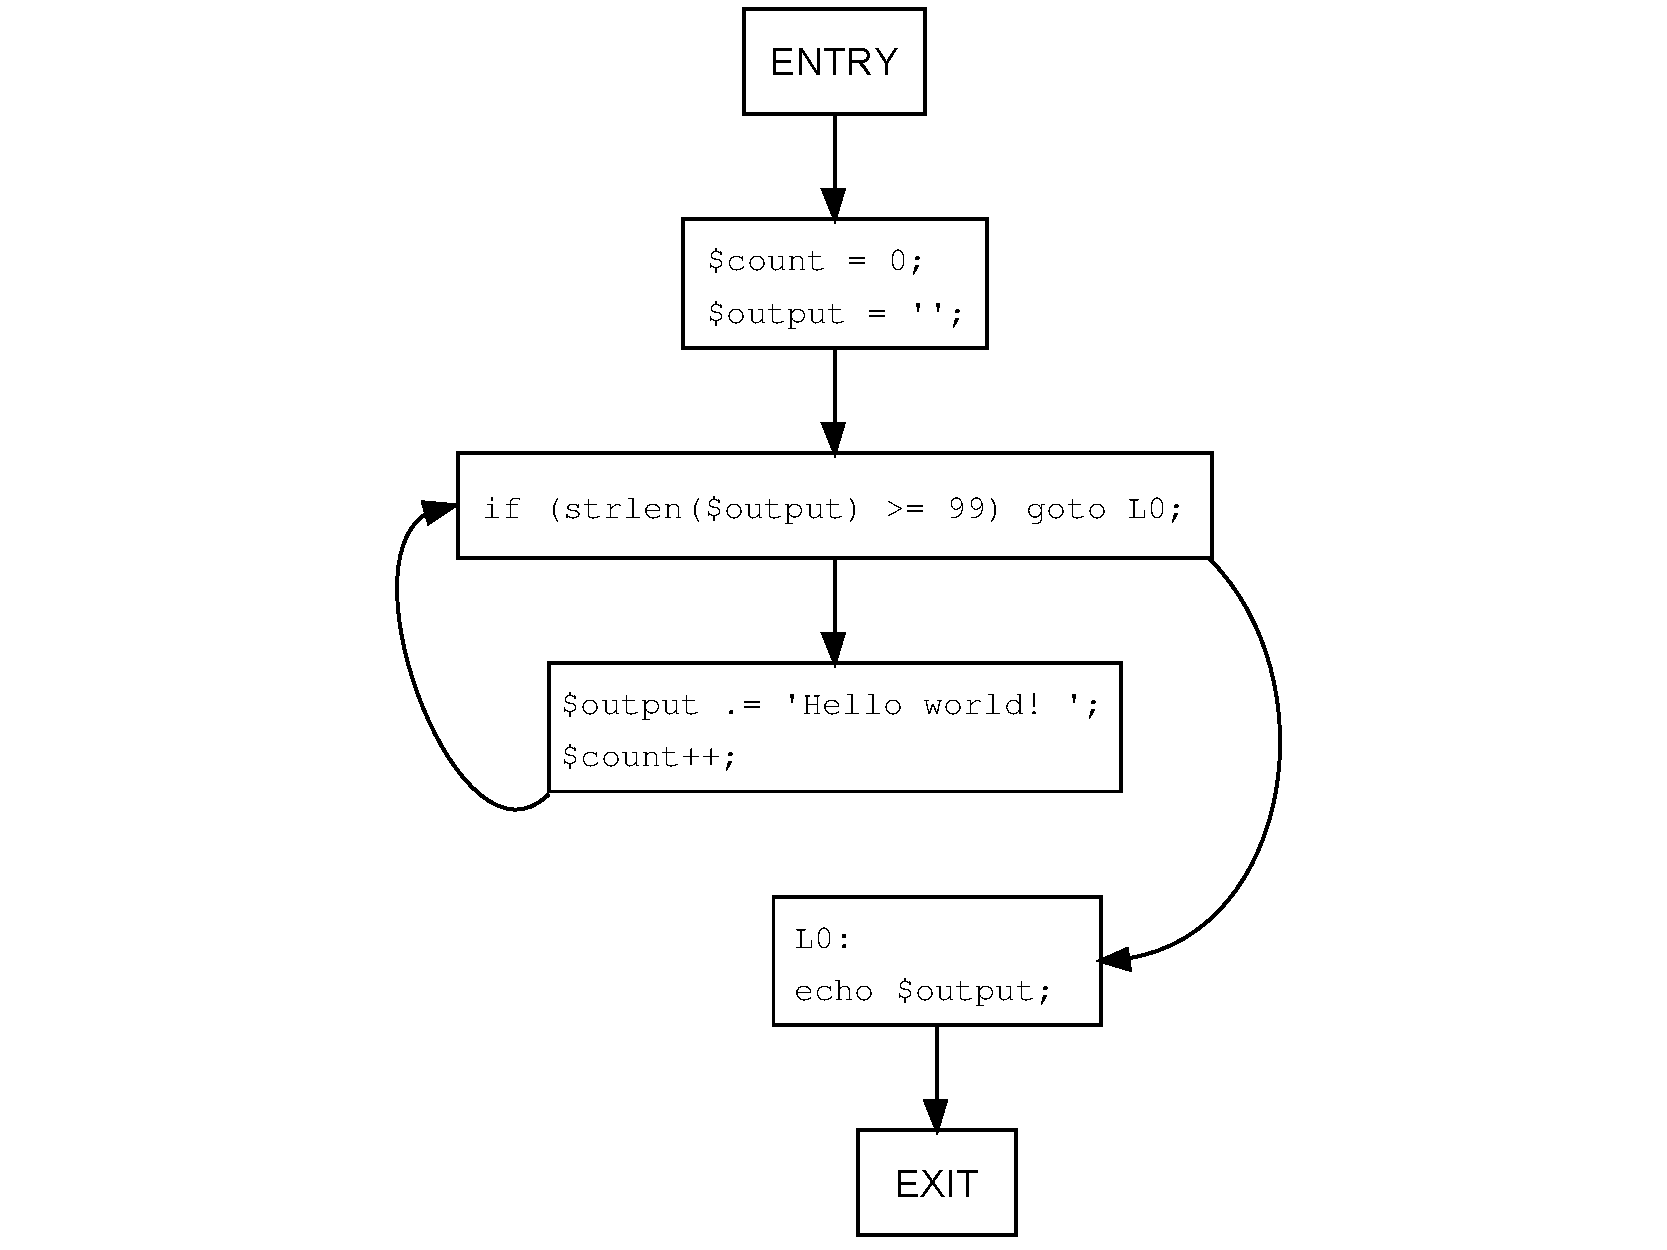
\includegraphics[scale=0.54, trim=10mm 0mm 0mm 0mm]{images/cfg}
    \caption{A control-flow graph represents all possible paths through a program.}
    \label{fig:cfg}
  \end{center}
\end{figure}

There are two special nodes in this graph---called \emph{ENTRY} and \emph{EXIT}. Those nodes do not represent any executable code, but are mere markers for the control-flow. The \emph{ENTRY} must not have any incoming edges, and the \emph{EXIT} nodes must not have any outgoing edges---actually, they are the only nodes without any outgoing edges. A control-flow graph may have only one entry node, but several exit nodes.

Note that a non-entry node without any incoming nodes is not reachable, \ie the code contained in that node is \emph{dead code}.

A node may contain several instructions. These multi-instruction nodes are called \emph{basic blocks}. However, an incoming edge can only point to a node, not to an individual instruction within a node. Thus, if an instruction is the target of the jump, the instruction needs to be the first one of a basic block.

The same goes for outgoing edges which can only be attached to a complete node, not to individual instructions within that node. Thus, if an instruction contains a jump, it needs to be the last instruction in a basic block, and the following instructions need to be placed within another basic block.

This allows for control-flow graphs to model all possible execution paths through a program in a way that each basic block either gets executed as a whole, or it does not get executed at all.



\section{Static Analysis for Finding Vulnerabilities}

Tools for static code analysis can find real bugs in production software \cite{findbugs, evaluating}, including security problems such as unintentionally ignored expressions, use-after-free~\cite{use-after-free-definition} or buffer overflows. Coverty~\cite{coverity-report}\index{Coverity} regularly uses their scanner to scan some open source projects for free, provide the bug reports to the projects, and publish regular reports on their efforts and the results, including numbers on the different vulnerability types found by their tool.

\cite{chess-west} explains in detail the way static analysis of code works and the techniques to use it to find bugs and vulnerabilities.



\section{Scanning for Tainted Object Propagation Problems}
\label{tainting}\index{tainted object propagation}\index{tainted object propagation scanners}

For finding \emph{tainted object propagation} problems (see section~\ref{tainted-object-propagation} on page~\pageref{tainted-object-propagation} for details), scanners use the approach described below.~\cite{finding-security-vulnerabilities, chess-west} This kind of scanner correspondingly is called \emph{tainted object propagation scanner}.

The scanner tracks where potentially untrusted data enters the application in places that are called \bb{sources}\index{source}, for example parts of the request. In the example (figure \ref{fig:taint} on page \pageref{fig:taint}), the \texttt{\$\_GET} variable ``name'' is a source.

The data is used during an \texttt{echo} call, outputting the data in the request body. Places like this in which data gets used in a way that could cause harm are called \bb{sinks}\index{sink}. In this case, the vulnerability would be \emph{cross-site-scripting (XSS)} (section~\ref{xss} on page~\pageref{xss}).

\begin{figure}[htb]
  \begin{center}
    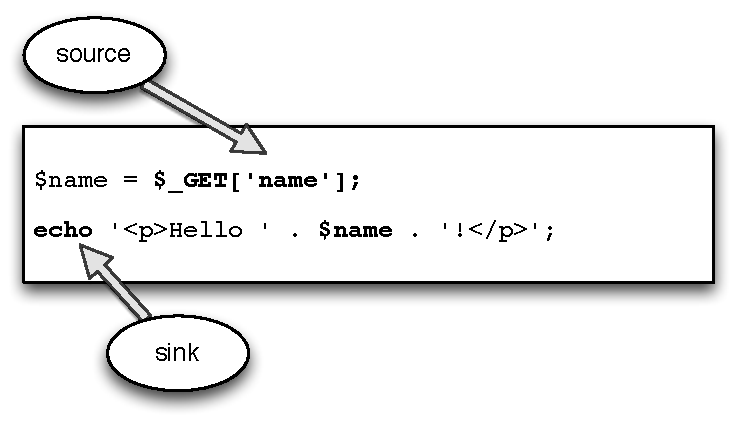
\includegraphics[scale=0.75]{images/taint}
    \caption{Tainted data enters the application via a \texttt{\$\_GET} variable source and gets used in an \texttt{echo} sink.}
    \label{fig:taint}
  \end{center}
\end{figure}

Sinks are specific to certain kinds of vulnerabilities. For example, the \texttt{echo} call is a sink for cross-site scripting, but it is not a sink for SQL injection~(section~\ref{sql-injection} on page~\pageref{sql-injection}), whereas a \texttt{mysql\_query} call is a sink for SQL injection, but not for cross-site scripting. Sources, however, are not vulnerability-specific---either the data from a source generally is to be trusted, or it is considered untrusted.

Data originating in a source (\ie untrusted data) is called \bb{tainted}\index{tainting} as long as it does not get \bb{sanitized}\index{sanitation}. In the second example (figure \ref{fig:taint-and-clean} on page \pageref{fig:taint-and-clean}), the \texttt{htmlspecialchars}\index{htmlspecialchars} call---which escapes all HTML entities---makes the tainted data safe in regards to cross-site scripting. Like sinks, sanitation is specific to certain kinds of vulnerabilities: For example, the \texttt{htmlspecialchars} call does not make the data safe concerning SQL injection.

Thus, a variable's \emph{taint state}\index{taint state}\label{taint-state} at some point of the program execution can either be \emph{tainted} or \emph{untainted}.

\begin{figure}[htb]
  \begin{center}
    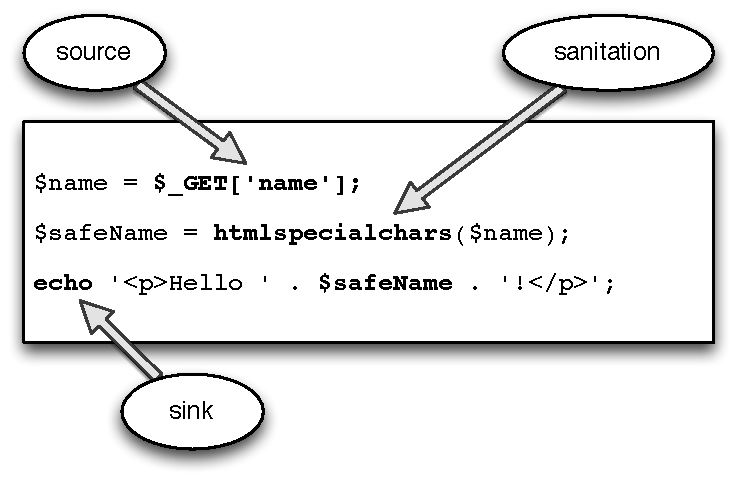
\includegraphics[scale=0.75]{images/taint-and-clean}
    \caption{Tainted data gets sanitized for XSS using \texttt{htmlspecialchars}.}
    \label{fig:taint-and-clean}
  \end{center}
\end{figure}

A tainted object propagation scanner uses data-flow analysis\index{data-flow analysis} to track the state of data (tainted or untainted in regard to certain vulnerability types) at each point of the program. When data flows into a sink for a certain type of vulnerability, and the data is tainted for this type of vulnerability, the scanner has found a vulnerability.

In their scanner \emph{Pixy}~\cite{pixy-short, pixy-long, pixy-dissertation}\index{Pixy}, the authors apply the tainted object propagation scanning approach to PHP.

In the author's experience in the TYPO3 security team~\cite{security-team-members}, most programmers have a rough understanding of the tainted object  propagation concept, but lack in understanding which sinks and which sanitation functions relate to what type of vulnerability. A common e-mail exchange about a vulnerable TYPO3 extension would go like this:

\begin{quote}

\bb{Security team member:} Dear TYPO3 extension author, an SQL injection vulnerability has been found in your extension and confirmed by our team. In line~172 of the file \texttt{foo.php}, data is read from a GET variable and then used for an SQL query in line~208 without being sanitized first.

Could you please send us a patch that fixes this issue together with an updated version of your extension?

\bb{TYPO3 extension author:} Thanks for your e-mail. Please find attached the patch and the new version of the extension.

\bb{Security team member:} (looks at the patch and finds an \texttt{htmlspecialchars} call that is supposed to fix the SQL injection) \emph{Sigh.}

\end{quote}
